\documentclass[a4paper,12pt]{article}

\usepackage{graphicx}
\usepackage{amsmath}
\usepackage{hyperref}
\usepackage{caption}
\usepackage{subcaption}
\usepackage{circuitikz}
\usepackage{longtable} 
\usepackage{tikz}

\title{\textbf{Lab Report: Experiment 2}}
\author{EE24BTECH11003 : Akshara Sarma Chennubhatla\\EE24BTECH11005 : Arjun Pavanje}

\begin{document}
\maketitle
\begin{center}
	\textbf{Experiment:}\\Studying the transient\\and steady state response\\of an RC Circuit\\with Square Wave Input
\end{center}
\vspace{30pt}
\begin{figure}[h!]
	\centering
	
\includegraphics[width = 100pt]{.logo/logo.png}\\
\end{figure}
\begin{center}
	Bachelor of Technology\\
	\vspace{10pt}
	Department of Electrical Engineering\\
\end{center}
\newpage

\section{Introduction}
In this experiment, we investigate the frequency response of the RC low-pass filter for single-stage, two-stage (cascade), and three-stage (cascade) filters. The objective is to derive the transfer function for each case and plot the Bode magnitude and phase responses. The components used in the experiment have the following values:
\begin{itemize}
    \item Resistance, $ R = 100 \, \Omega $
    \item Capacitance, $ C = 0.1 \, \mu F $
\end{itemize}

\section{Transfer Function and Bode Plot for Single-Stage RC Filter}

The transfer function of a single-stage RC low-pass filter is given by:

\begin{align*}
H(s) &= \frac{V_{\text{out}}(s)}{V_{\text{in}}(s)} = \frac{1}{1 + sRC}
\end{align*}

Where:
\begin{itemize}
    \item $ R $ is the resistance,
    \item $ C $ is the capacitance,
    \item $ s = j\omega $ is the complex frequency.
    \item $X_c = \frac{1}{j\omega C}$ is the impedance due to capacitor
\end{itemize}

\subsection{One-Stage RC Low-Pass Filter}
\pagebreak
\begin{figure}[!h]
\centering
\resizebox{1\textwidth}{!}{%
\begin{circuitikz}
\tikzstyle{every node}=[font=\normalsize]
\draw (5,14.5) to[sinusoidal voltage source, sources/symbol/rotate=auto] (5,10.75);
\draw (5,14.5) to[R,l={ \normalsize R}] (8.75,14.5);
\draw (8.75,14.5) to[C,l={ \normalsize C}] (8.75,10.75);
\draw (8.75,10.75) to[short] (5,10.75);
\draw (8.75,14.5) to[short, -o] (10.25,14.5) ;
\draw (8.75,10.75) to[short, -o] (10.25,10.75) ;
\node [font=\normalsize] at (4,12.75) {$V_{in}$};
\node [font=\normalsize] at (5,14.75) {$a$};
\node [font=\normalsize] at (8.75,14.75) {$b$};
\node [font=\normalsize] at (11,12.75) {$V_{out}$};
\draw [<->, >=Stealth] (10.25,11) -- (10.25,14.25);
\end{circuitikz}
}%
\label{one-cascade}
\end{figure}
Applying $KVL$ at node $b$
\begin{align*}
    \frac{\vec{v}_{out} - \vec{v}_{in}}{R} + \frac{\vec{v}_{out}}{X_c} &= 0
\end{align*}
We get, 
\begin{align*}
    \vec{v}_{out} \left( \frac{R+X_c}{X_c} \right) = \vec{v}_{in}\\
    H(jw) =  \frac{1}{1+j\omega RC}
\end{align*}
We finally get,
\begin{align*}
    |H(jw)| &= \frac{1}{\sqrt{1 + \omega^2 R^2 C^2}}\\
    \phi &= -\tan^{-1}\left( \omega RC\right)
\end{align*}

\subsection{Two-Stage RC Low-Pass Filter (Cascade of Two Filters)}
\pagebreak
\begin{figure}[!h]
\centering
\resizebox{1\textwidth}{!}{%
\begin{circuitikz}
\tikzstyle{every node}=[font=\normalsize]
\draw (5,14.5) to[sinusoidal voltage source, sources/symbol/rotate=auto] (5,10.75);
\draw (5,14.5) to[R,l={ \normalsize R}] (8.75,14.5);
\draw (8.75,14.5) to[C,l={ \normalsize C}] (8.75,10.75);
\draw (8.75,10.75) to[short] (5,10.75);
\node [font=\normalsize] at (4,12.75) {$V_{in}$};
\draw (8.75,14.5) to[R,l={ \normalsize R}] (12.5,14.5);
\draw (12.5,14.5) to[C,l={ \normalsize C}] (12.5,10.75);
\draw (12.5,10.75) to[short] (8.75,10.75);
\draw (12.5,14.5) to[short, -o] (14,14.5) ;
\draw (12.5,10.75) to[short, -o] (14,10.75) ;
\node [font=\normalsize] at (14.75,12.5) {$V_{out}$};
\draw [<->, >=Stealth] (14,11) -- (14,14.25);
\node [font=\normalsize] at (5,14.75) {$a$};
\node [font=\normalsize] at (8.75,14.75) {$b$};
\node [font=\normalsize] at (12.5,14.75) {$c$};
\end{circuitikz}
}%
\label{2 cascade}
\end{figure}
Applying $KVL$ at node $c$
\begin{align*}
    \frac{\vec{v}_{out}}{X_c} + \frac{\vec{v}_{out} - \vec{v}_b}{R} = 0\\
    \vec{v}_b = \vec{v}_{out}\left(\frac{R+X_c}{X_c}\right)
\end{align*}
Applying $KVL$ at node $b$
\begin{align*}
    \frac{\vec{v}_b - \vec{v}_{out}}{R} + \frac{\vec{v}_b}{X_c} + \frac{\vec{v}_b - \vec{v}_{in}}{R} = 0\\
    \vec{v}_{out}\left(\frac{R}{X_c}\right) + \vec{v}_{out}\left(\frac{R^2+RX_c}{X_c^2}\right) + \vec{v}_{out}\left(\frac{R+X_c}{X_c} \right) = \vec{v}_{in}\\
    \vec{v}_{out}\left(\frac{R^2 + X_c^2 + 3RX_c}{X_c^2}\right)  = \vec{v}_{in}  
\end{align*}
The transfer function becomes:

\begin{align*}
H(j\omega) = \frac{1}{(1-\omega^2R^2C^2) + j(3\omega RC)}
\end{align*}
We finally get,
\begin{align*}
    |H(jw)| &= \frac{1}{\sqrt{(1 - \omega^2 R^2 C^2)^2 +(3\omega RC)^2}}\\
    \phi &= -\tan^{-1}\left( \frac{3\omega RC}{1-\omega^2R^2C^2}\right)
\end{align*}
\subsection{Three-Stage RC Low-Pass Filter (Cascade of Three Filters)}
\pagebreak
\begin{figure}[!h]
\centering
\resizebox{1\textwidth}{!}{%
\begin{circuitikz}
\tikzstyle{every node}=[font=\normalsize]
\draw (5,14.5) to[sinusoidal voltage source, sources/symbol/rotate=auto] (5,10.75);
\draw (5,14.5) to[R,l={ \normalsize R}] (8.75,14.5);
\draw (8.75,14.5) to[C,l={ \normalsize C}] (8.75,10.75);
\draw (8.75,10.75) to[short] (5,10.75);
\node [font=\normalsize] at (4,12.75) {$V_{in}$};
\draw (8.75,14.5) to[R,l={ \normalsize R}] (12.5,14.5);
\draw (12.5,14.5) to[C,l={ \normalsize C}] (12.5,10.75);
\draw (12.5,10.75) to[short] (8.75,10.75);
\draw (12.5,14.5) to[R,l={ \normalsize R}] (16.25,14.5);
\draw (16.25,14.5) to[C,l={ \normalsize C}] (16.25,10.75);
\draw (16.25,10.75) to[short] (12.5,10.75);
\draw (16.25,14.5) to[short, -o] (17.75,14.5) ;
\draw (16.25,10.75) to[short, -o] (17.75,10.75) ;
\node [font=\normalsize] at (18.5,12.5) {$V_{out}$};
\draw [<->, >=Stealth] (17.75,11) -- (17.75,14.25);
\node [font=\normalsize] at (5,14.75) {$a$};
\node [font=\normalsize] at (8.75,14.75) {$b$};
\node [font=\normalsize] at (12.5,14.75) {$c$};
\node [font=\normalsize] at (16.25,14.75) {$d$};
\end{circuitikz}
}%

\label{3 cascade}
\end{figure}
Applying $KVL$ on node $d$,
\begin{align*}
\frac{\vec{v}_{out} - \vec{v}_c}{R} + \frac{\vec{v}_d}{X_c} = 0 \\
\vec{v}_{out} \left( \frac{X_c + R}{X_c} \right) = \vec{v}_c  
\end{align*}
Applying $KCL$ on node $c$ we get,
\begin{align*}
    \frac{\vec{v}_c - \vec{v}_d}{R} + \frac{\vec{v}_c - \vec{v}_b}{R} + \frac{\vec{v}_c}{X_c} = 0\\
   \vec{v}_c = \vec{v}_{out} \left(\frac{(R+Z_c)^2 + RX_c}{X_c^2} \right)
\end{align*}
Applying $KVL$ on node $b$,
\begin{align*}
    \frac{\vec{v}_b - \vec{v}_{in}}{R} + \frac{\vec{v}_b - \vec{v}_c}{R} + \frac{\vec{v}_b}{X_c} = 0
\end{align*}
On simplifying we get,
\begin{align*}
    \vec{v}_{out} \left(\frac{RX_c(R+X_c) + (R + X_c)^3}{X_c^3} + \frac{R}{X_c} + \frac{R (X_c + R)}{X_c^2} \right) = \vec{v}_{in}\\
    \vec{v}_{out} \left(\frac{2RX_c(R+X_c) + (R + X_c)^3 + RX_c^2}{X_c^3}\right) = \vec{v}_{in}
\end{align*}
The transfer function becomes:

\begin{align*}
H(j\omega) = \frac{1}{(1-5\omega^2R^2C^2) + j(6\omega RC - \omega^3R^3C^3)}
\end{align*}
We finally get,
\begin{align*}
    |H(jw)| &= \frac{1}{\sqrt{(1 - 5\omega^2 R^2 C^2)^2 +(6R\omega C - \omega^3R^3C^3)^2}} \\
    \phi &= -\tan^{-1}\left( \frac{6\omega RC- \omega^3R^3c^3}{1-5\omega^2R^2C^2}\right)
\end{align*}
\section{Bode Plot Analysis}
The Bode plot is typically plotted in two parts: magnitude and phase\\

\textbf{Magnitude:}\\
$20$ $log_{10}(|H(jw)|)$ vs $log_{10}(w)$ is plotted\\

\textbf{Phase:}\\
$\phi$ vs $log_{10}(w)$ is plotted\\

The frequency response will be plotted for single, two-stage, and three-stage filters.

\section{Experimental Data}
One thing to note is that when the value of capacitance was verified using a multimeter, capacitance was found to be $0.88$ times the labelled value. So capacitance for theoretical calculations was taken to be $0.088 \mu F$. \\
The following table summarizes the experimental data collected. It includes the frequency ($f$), the magnitude of the transfer function $H(j\omega)$, and the change in the time ($\Delta t$)\\
One stage RC low pass filter:\\
\begin{longtable}{|c|c|c|}
\hline
\textbf{Frequency (Hz)} & \textbf{$|H(j\omega)|$} & \textbf{$\Delta t$} \\
\hline
\endfirsthead
\hline
\textbf{Frequency (Hz)} & \textbf{$|H(j\omega)|$} & \textbf{$\Delta t$} \\
\hline
\endhead
\hline
\endfoot
\hline
\endlastfoot
% Add experimental data here
50 & 0.96 & 0 \\
100 & 0.96 & 0 \\
200 & 0.96 & 0 \\
400 & 0.96 & 0 \\
800 & 0.96 & 0 \\
1600 & 0.96 & 3 \\
3200 & 0.94 & 4 \\
6400 & 0.88 & 8 \\
12800 & 0.77 & 6.4 \\
25600 & 0.55 & 5.6 \\
51200 & 0.34 & 3.6 \\
% continue adding your data
\end{longtable}
\pagebreak
Two stage RC low pass filter:\\
\begin{longtable}{|c|c|c|}
\hline
\textbf{Frequency (Hz)} & \textbf{$|H(j\omega)|$} & \textbf{$\Delta t$} \\
\hline
\endfirsthead
\hline
\textbf{Frequency (Hz)} & \textbf{$|H(j\omega)|$} & \textbf{$\Delta t$} \\
\hline
\endhead
\hline
\endfoot
\hline
\endlastfoot
% Add experimental data here
50 & 0.96 & 0 \\
100 & 0.96 & 0 \\
200 & 0.96 & 0 \\
400 & 0.96 & 5 \\
800 & 0.96 & 10 \\
1600 & 0.96 & 24 \\
3200 & 0.916 & 18 \\
6400 & 0.77 & 16 \\
12800 & 0.55 & 14 \\
25600 & 0.277 & 10 \\
51200 & 0.13 & 6 \\
% continue adding your data
\end{longtable}
Three stage RC low pass filter:\\
\begin{longtable}{|c|c|c|}
\hline
\textbf{Frequency (Hz)} & \textbf{$|H(j\omega)|$} & \textbf{$\Delta t$} \\
\hline
\endfirsthead
\hline
\textbf{Frequency (Hz)} & \textbf{$|H(j\omega)|$} & \textbf{$\Delta t$} \\
\hline
\endhead
\hline
\endfoot
\hline
\endlastfoot
% Add experimental data here
50 & 0.9615 & -19.8 \\
100 & 0.96 & -9.85 \\
200 & 0.96 & -5 \\
400 & 0.96 & -2.47 \\
800 & 0.96 & -1.22 \\
1600 & 0.92 & -0.57 \\
3200 & 0.833 & -0.282 \\
6400 & 0.651 & -0.13 \\
12800 & 0.409 & -0.053 \\
25600 & 0.203 & -0.025 \\
51200 & 0.03 & -0.0105 \\
% continue adding your data
\end{longtable}
\section{Plots}
\subsection{One Stage:}
\pagebreak
\begin{figure}[h!]
	\begin{subfigure}[b]{100pt}
		\caption{Magnitude plot}
		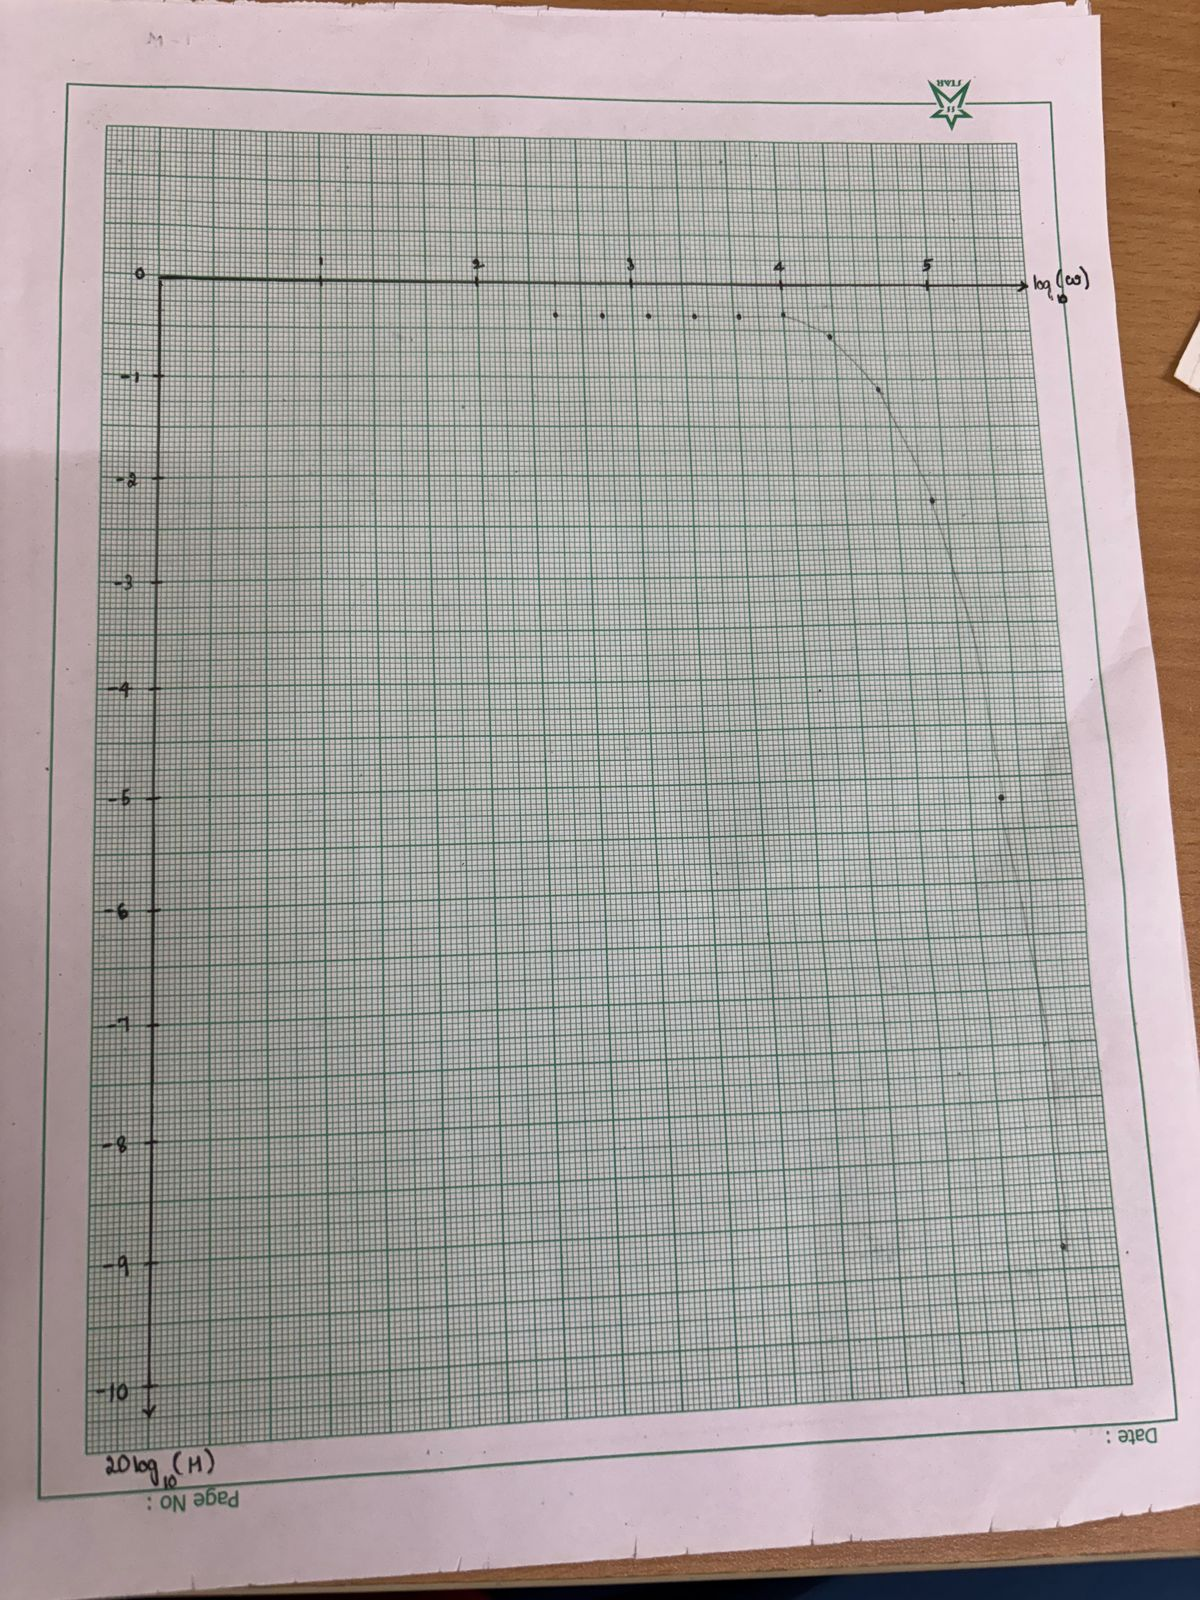
\includegraphics[width = 230pt]{figs/fig1.png}
	\end{subfigure}
	\hspace{110pt}
	\begin{subfigure}[b]{100pt}
		\caption{Phase plot}
		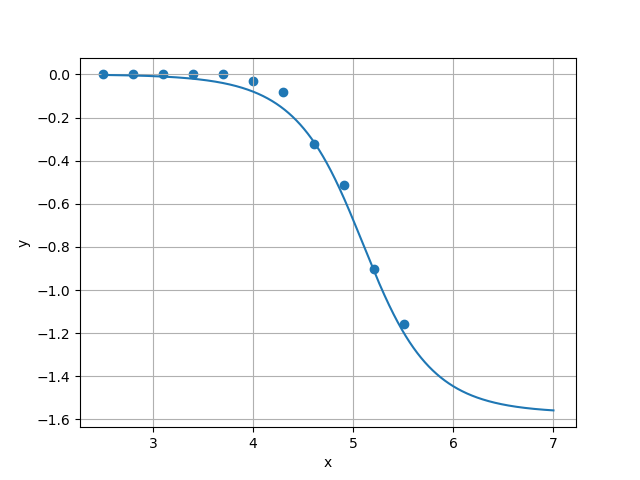
\includegraphics[width = 225pt]{figs/fig2.png}
	\end{subfigure}
\end{figure}
\subsection{Two Stage:}
\pagebreak
\begin{figure}[h!]
	\begin{subfigure}[b]{100pt}
		\caption{Magnitude plot}
		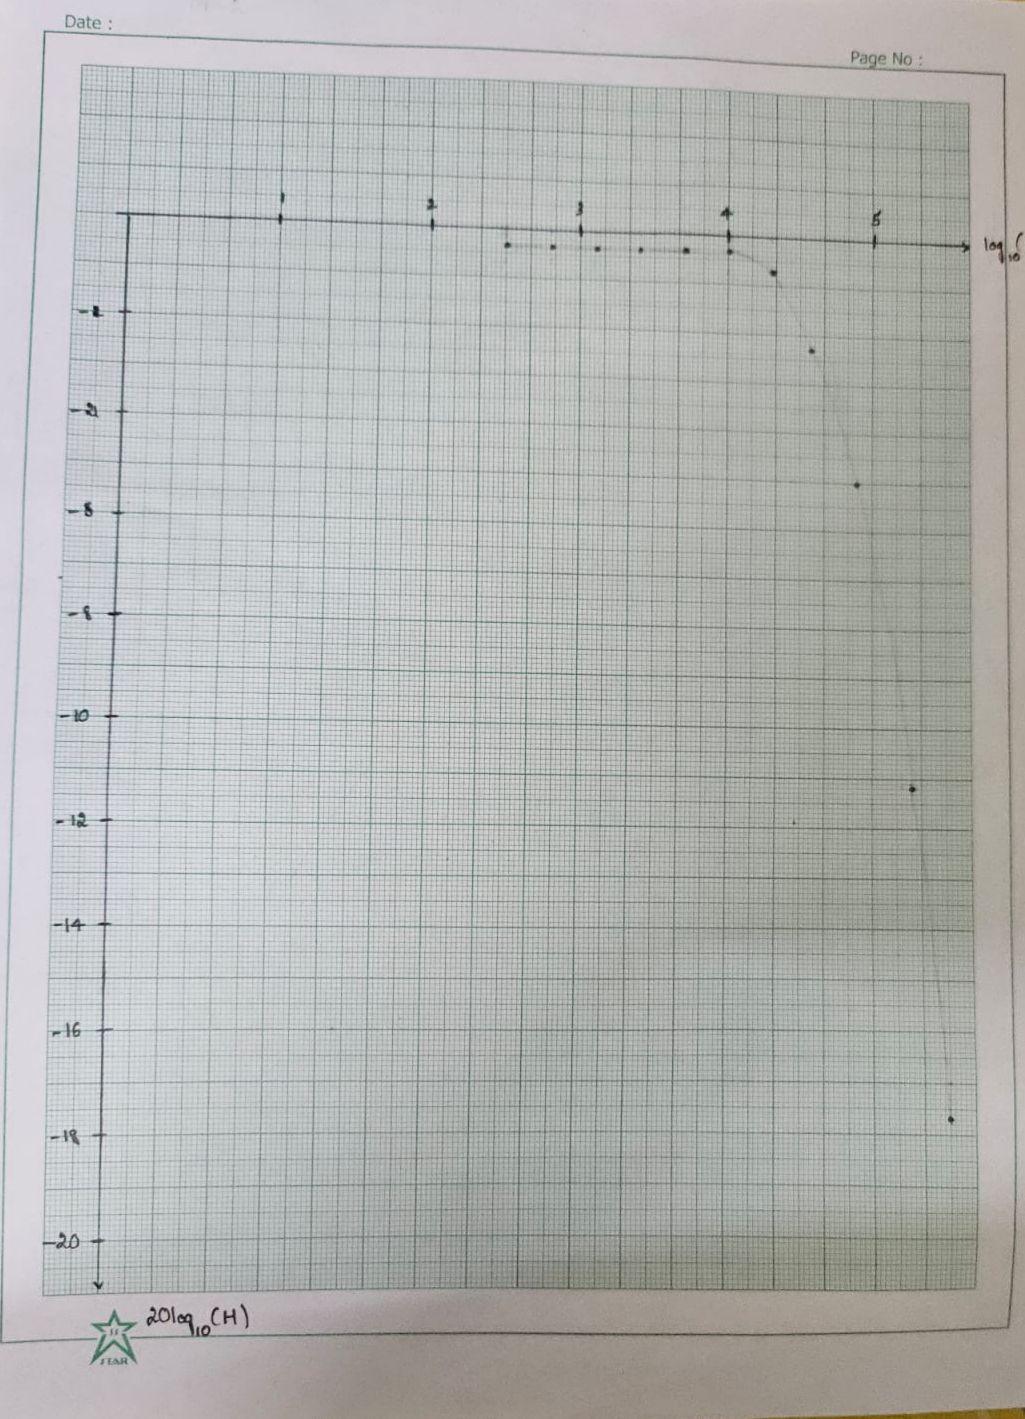
\includegraphics[width = 215pt]{figs/fig3.png}
	\end{subfigure}
	\hspace{110pt}
	\begin{subfigure}[b]{100pt}
		\caption{Phase plot}
		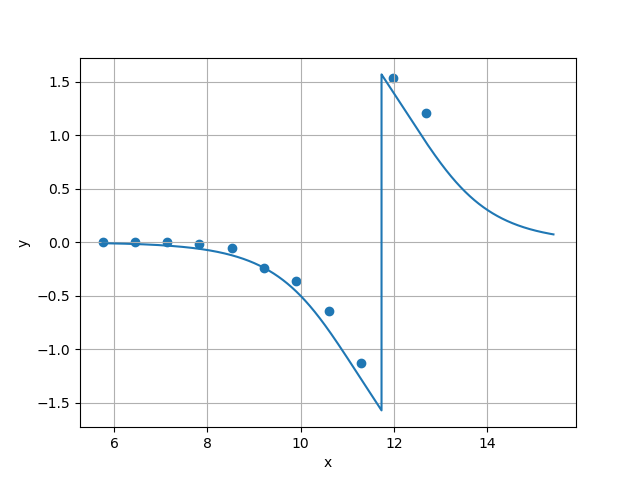
\includegraphics[width = 230pt]{figs/fig4.png}
	\end{subfigure}
\end{figure}
\subsection{Three Stage:}
\pagebreak
\begin{figure}[h!]
	\begin{subfigure}[b]{100pt}
		\caption{Magnitude plot}
		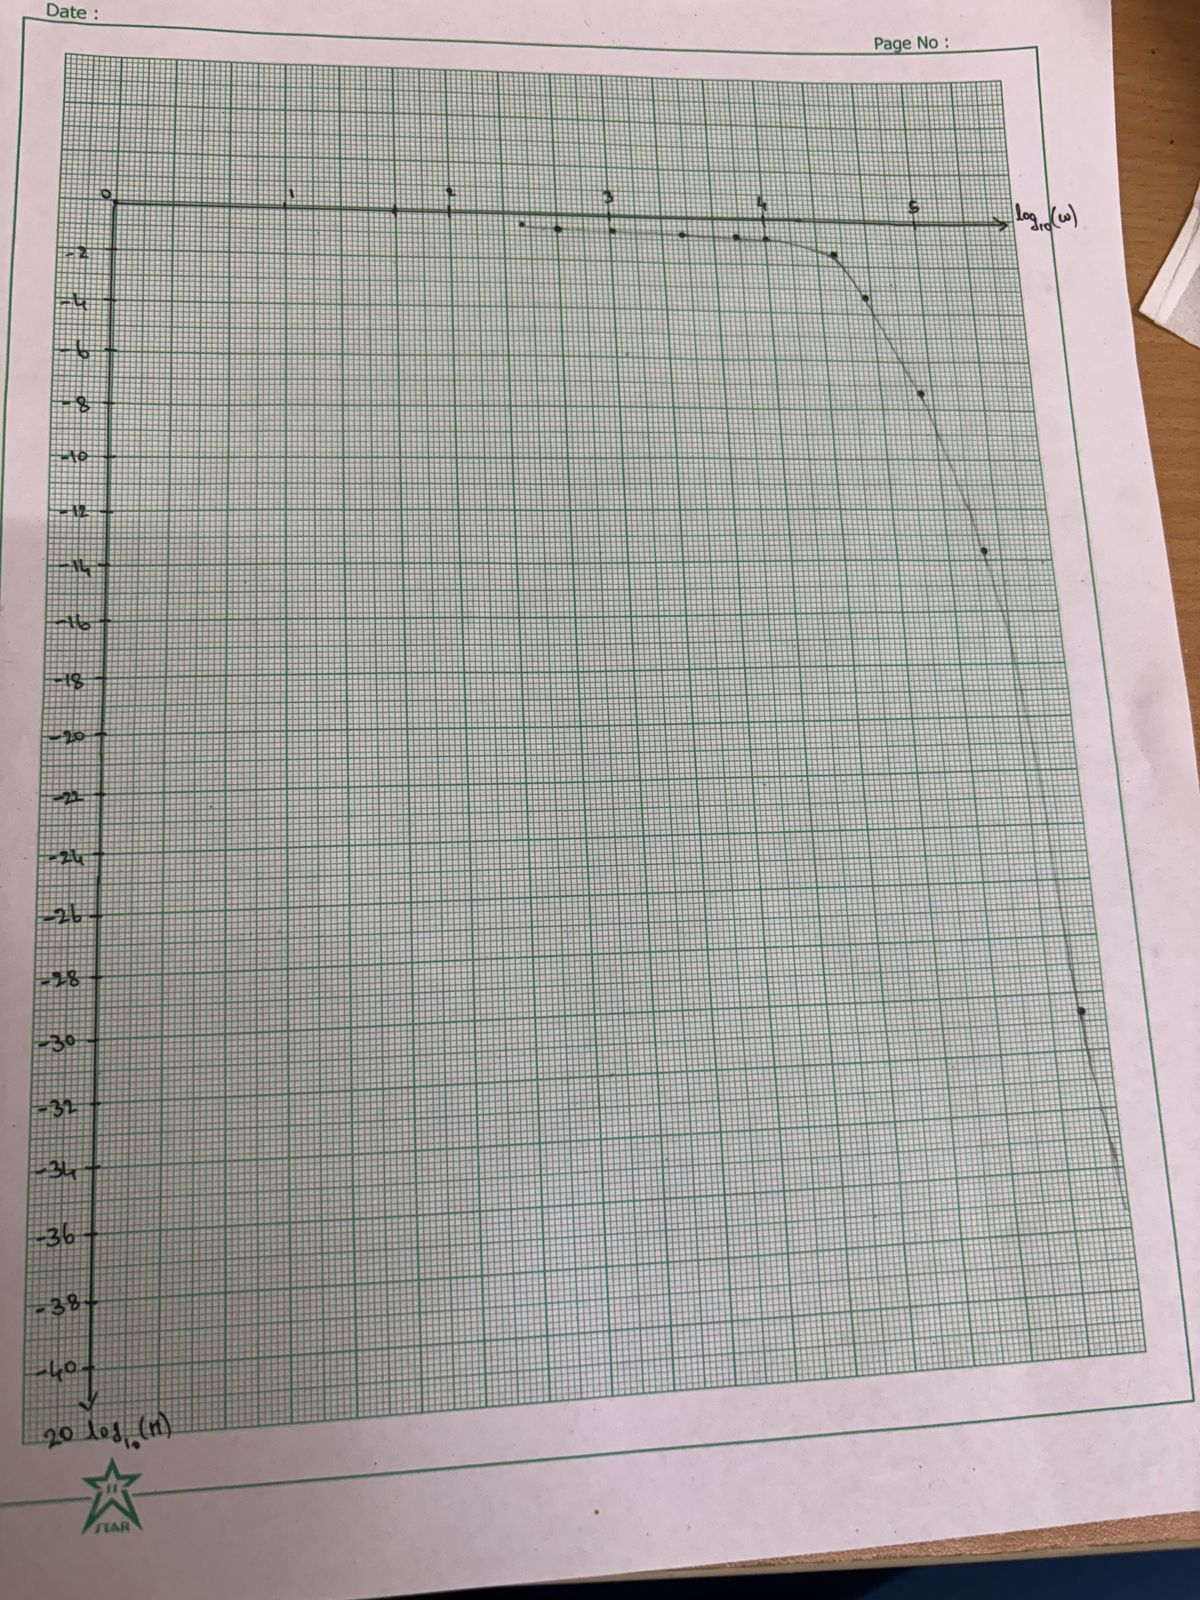
\includegraphics[width = 230pt]{figs/fig5.png}
	\end{subfigure}
	\hspace{110pt}
	\begin{subfigure}[b]{100pt}
		\caption{Phase plot}
		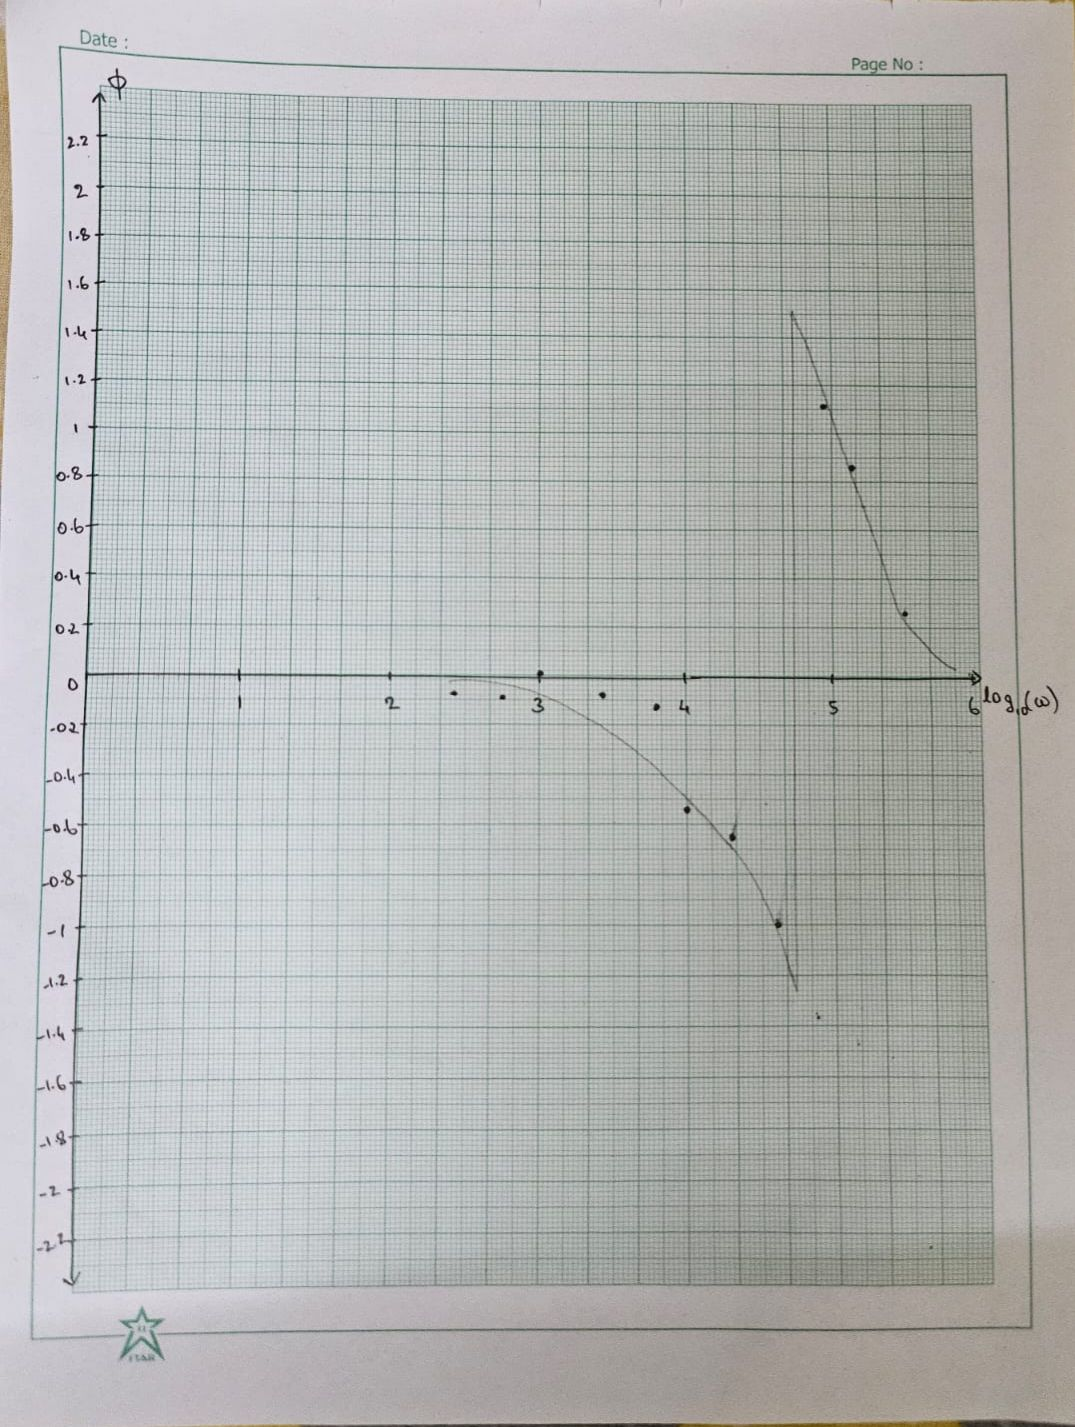
\includegraphics[width = 228pt]{figs/fig6.png}
	\end{subfigure}
\end{figure}
If images are not clear,\\
\fbox{\url{https://github.com/ArjunPavanje/EE1200/tree/main/Experiment_3/figs}}\\\\
To view theoretical verifcation of obtained data,\\
\fbox{\url{https://github.com/ArjunPavanje/EE1200/tree/main/Experiment_3/codes}}
\section{Conclusion}
In this experiment, we derived the transfer functions for single-stage, two-stage, and three-stage RC low-pass filters, analyzed the frequency response, and generated Bode plots for each case. The cascade of stages leads to a steeper roll-off in the frequency response as the number of stages increases.

\end{document}
